\documentclass[10pt,a4paper]{article}
\usepackage[english]{babel}
\usepackage{amsmath}
\usepackage{graphicx}
\usepackage{lmodern}
\usepackage[font=small,format=plain,labelfont=bf,up,textfont=it,up]{caption}
\usepackage[nottoc]{tocbibind}
\usepackage{url}
\usepackage{courier}
\usepackage[T1]{fontenc}
\usepackage[titles]{tocloft}
\usepackage{subfig}

\setcounter{secnumdepth}{5}
\setlength{\parindent}{0in}

\renewcommand{\topfraction}{0.85}
\renewcommand{\textfraction}{0.1}
\renewcommand{\floatpagefraction}{0.75}

\makeatletter
\newcommand\ackname{Acknowledgements}
\if@titlepage
  \newenvironment{acknowledgements}{
      \titlepage
      \null\vfil
      \@beginparpenalty\@lowpenalty
      \begin{center}%
        \bfseries \ackname
        \@endparpenalty\@M
      \end{center}}%
     {\par\vfil\null\endtitlepage}
\else
  \newenvironment{acknowledgements}{
      \if@twocolumn
        \section*{\abstractname}
      \else
        \small
        \begin{center}
          {\bfseries \ackname\vspace{-.5em}\vspace{\z@}}
        \end{center}
        \quotation
      \fi}
      {\if@twocolumn\else\endquotation\fi}
\fi
\makeatother

\title{CuEira, gene-enviroment interaction analysis on GPU}
\author{Daniel Berglund}
\date{March 2014}

\begin{document}
\maketitle
\thispagestyle{empty}

\clearpage
\thispagestyle{empty}
\selectlanguage{english}
\begin{abstract}
Abstract in english
\end{abstract}

\clearpage
\thispagestyle{empty}
\selectlanguage{english}
\begin{abstract}
Abstract på svenska
\end{abstract}

\clearpage
\thispagestyle{empty}
%\begin{acknowledgements}
%Asdf
%\end{acknowledgements}

%\clearpage
\thispagestyle{empty}
\tableofcontents

\newpage
\setcounter{page}{1}
\section{Introduction}
%\subsection{Epidemiology}
%Epidemiology is the study of 

%It combines

%\cite{rothman1998modern,rothman2002intro_epidemiology}

\subsection{Genome-wide association studies}
Genome-wide association studies(GWAS) is a common type of study to search for associations between genetic markers and diseases. Classicaly it doesn't consider interaction between the genetic markers nor enviromental factors. Gene-gene interaction has started to become more common\cite{cordell_detect_review}, however gene-enviroment is still uncommon\cite{gene_enviroment_2013}. Interaction between genes and enviromental factors are considered imporant for complex diseas such as cancer and autoimmune diseases.\cite{cordell_detect_review, gene_enviroment_2013, geira, ra_smoking}\\
\\
These types of studies are usually either cohort or case-control. In cohort studies a sample of a population who don't have the disease is followed. Variables that are suspected to be releveant for the disease is measured and over time some of the individuals will get the disease. The data collected can then be used to find risk factors. In case-control studies two groups are compared to find risk factors. One group consists of individuals with the disease and the other of individuals that are similar to the cases but that doesn't have the disease.\cite{rothman1998modern,mann_observational}\\
\\
The genetic markers are commonly single-nucleotide polymorphisms(SNPs). SNPs are variations in the genome where a single nucleotide differs between individuals in a population\cite{fareed_snp}. Enviromental factors can be various things such as smoking, physical activity and so on. The amount of data is usually thousands individuals and hundred thousands or millions SNPs. Due to the high number of SNPs few programs investigate more than second order interaction. There are some that can handle more however they have drawbacks\cite{gwis,high_order_2012,fast_high_order_cluster}.

\subsection{High Performance Computing}
High Performance Computing(HPC) is a branch of computer science that focuses on developing supercomputers and related software. Since they are parallel a big area is how to parallelize various algorithms. In HPC groups of computers called \emph{clusters} are used.\cite{intro_hpc, introduction_hpc_hager}

Moores Law, more threads, increased need for parallelization
Plot of speed without increased number of cores and with

However HPC is more than just flops/sec, especially since other parts of the computers aren't improving as fast as the compuing power. Few applications today is even near peak performance due to various latency and bandwidth problems.

\subsection{Defining Interaction}
What do we mean with interaction between factors? There are several definitions of the term\cite{rothman2002intro_epidemiology}. The overall goal is usually to find if \emph{biological} interaction is present. Biological interaction is when the factors co-operate through a physiological or biological mechanism and causes the effect, eg. disease. This is useful since it's the true interaction in some sense and we can use it to explain the mechanisms involved and possibly find cures for diseases. However it's not well defined, it's not something we can calculate directly from data.\cite{rothman1998modern,rothman2002intro_epidemiology}\\
\\
\emph{Statistic} interaction on the other hand is well defined. However it's scale dependant, ie. interactions can appear and disappear based on transformations of the data. It also depends on the model used, eg Logistic, Linear. The common way to define statistic interaction is as the presence of product terms between the factors in the statistical model, this is refred to as \emph{multiplicative} interaction. For instance for a linear model
$$f(x,y)=ax+by+cxy+d$$
c is the product term that represents multiplicative interaction between variables x and y. Statistic interaction is often called just interaction which can make it a  bit confusig.\cite{geira,rothman1998modern}\\
\\
It can also be defined as the divergence from additeve effects

It's called biological interaction by Rothman\cite{rothman1998modern} and can also be called \emph{additive} interaction\cite{geira}. Here we we will use the term \emph{causual} interaction\cite{causal_bounds_arvid}.\\

%Something about sufficnt cause?

\subsection{GEIRA and JEIRA}
GEIRA is a tool for analysing gene-gene and gene-enviroment interaction. GEIRA uses additive interaction instead of multiplicative, commonly multiplicative interaction is used\cite{geira}. JEIRA is a parallelized immplementation of the enviromental interaction analysis in GEIRA. However it can only use one node.

\clearpage
\section{Background}
%Mathematical and physical bck (equations etc.)
%Algorithmic bck and concepts (e.g scalability, speedup etc.)
%computer architecture bck(describe CPU and GPU differences etc.)
Most research have focused on gene-gene interaction so there are few tools for gene-enviroment. SNPs are binary variables which is an advantage that is almost always used when searching for gene-gene interaction. They are binary since the three possible combinations of allels(AA, Aa, aa)  can be represtend as 1,1,0 if its dominat model and 0,0,1 if its ressive\cite{}. Enviromental factors can be of any type\cite{gene_enviroment_2013}. Gene-gene interaction tools can sometimes be used to find gene-enviroment interaction, however they usually require the variable to be binary or have other problems since they weren't designed for gene-enviroment interaction.\cite{gene_enviroment_2013}\\ %Studies involving enviromental factors also have the can also change over time(eg a person can stop smoking, move to a different area) while a persons genome reamains more or less constant.
\\
Both CPU clusters\cite{biforce} and GPUs\cite{gwis,gboost,gmdr_gpu,cuda_lr,genie_2012,plink_gpu}, in some cases GPU clusters\cite{gwis_conf} have been used for GWAS. GPUs have been a popular choice since most of the methods for searching for interaction are inherintly good on GPUs because each combination can usually be considered independently from the others. More about this in the section \ref{gpu_gwas}.\\
\\
There are a lot of algorithms and programs proposed for searching for interaction, most have focused on binary variables as already mentioned. They can be roughly classiefed into four categories, exhaustive, stochastic, machine learning/data mining and stepwise\cite{fast_high_order_cluster}. One of the differences between methods is wether they are testing for interaction or testing for allowing interaction, see section \ref{test_type} for details. In short it's testing if there is interaction or if there is an effect from either factor or from interaction.\\
\\
Exhaustive search is the most direct approach, they compare all combinations of the SNPs in the data. They don't risk missing a combination but it also means they can be slow. Multifactor-Dimensionality Reduction(MDR)\cite{mdr_2001} and BOOST\cite{boost_gene_gene} are two examples.\\
\\
Stochastic methods uses random sampling to ``walk'' through the data. BEAM\cite{beam_2007} is one example and it uses Markov Chain Monte Carlo(MCMC).\\
\\
Machine Learning and Data Mining methods are methods from computer science. They are methods learn from data and tries to generalize it. MDR\cite{mdr_2001} is the among the most common methods used in GWAS that is a computer science approach. See section \ref{data_machine_learning} for more details.\\
\\
Stepwise approaches uses a filtering stage and a search stage. At the filtering stage uninterestings combinations are filtered out by using some exhaustive method. The other SNPs are the examined more carefully in the search stage. BOOST\cite{boost_gene_gene} is an example which uses clever datastructures and a likelihood ratio test to filter the data.

\subsection{Confounders and Covarietes}
Confounding is one of the central issues in the design of epidemiologic studies. It's when the effect of the exposure is mixed with the effect of another variable. So if we don't measure the second variable the first effect would be estimated as stronger than it really is. The second varialbe is then a \emph{confounder}. Several methods in epidemiology are about avoiding or adjusting for confounding. Sometimes these variables needs to be incorperated into the models. Covarietes are possible confounders or other variables that you want to adjust for in the model. Somtimes covariets are called control variables.\cite{rothman2002intro_epidemiology,rothman1998modern}

\begin{figure}[h]
    \centering
    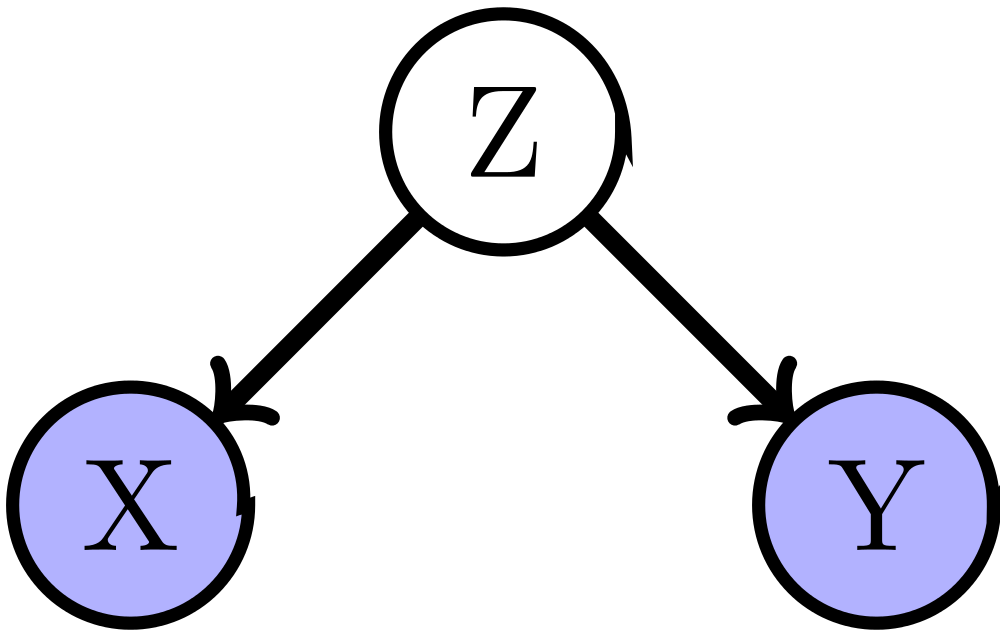
\includegraphics[width=5cm]{Simple_Confounding_Case.png}
    \caption{Illustration of a simple case of confounding. If we don't observe Z we might falesly find an association between X and Y. Wikipedia Commons}
    \label{fig:confunding}
\end{figure}

\subsection{The Multiple Testing Problem}
It's not uncommon to test a lot of hypothesis on the same data and in the case of GWAS it can be billions of tests. If we continue testing we should eventually find something that is significant. Also rember that the standard p-value of 5\% means that we expect to find 1 in 20 false positives under the assumption that the null hypothesis is true. The problem arise from the fact that the hypothesis tests are dependent on each other since they use parts of the same data.. This is the multiple testing problem and if it's not corrected for we might find a lot of fale positives.\cite{bonferroni_multiple}\\
\\
Bonferroni correction is the simplest and viewed as the most conservative way to correct for this problem, simply divided the p-value threshold that a tests passes with the number of hypothesis. However how many hypothesis that are made isn't always obvious. For instance for a two stage analysis. Is the number of hypothesis the number of tests done in both stages combined, the number made in the first stage or the second stage?\cite{bonferroni_multiple}

\subsection{Contingency Tables}
A contingency table is a matrix used to describe categorical data. Each cell contains the frequency of occurances with a specific combination of variables. Table \ref{table:contingency_table} is an example of an 2 x 3 table. From it we can for instance see that 171 persons that got the placebo had an nonfatal attack. Contingency tables are the basis for various statistical tests to model the data. Contingency tables can be used directly for tests like $chi^2$.\cite{agresti_categorical}

\begin{table}[h]
\begin{tabular}{ l c c c }
  \hline
  & Fatal Attack & Nonfatal Attack & No Attack\\
  \hline
  Placebo & 18 & 171 & 10 845 \\
  Aspirin & 5 & 99 & 10 933 \\
  \hline  
\end{tabular}
\caption{Contingency table describing the outcome of a medical study, from \cite{agresti_categorical}}
\label{table:contingency_table}
\end{table}

\subsubsection{Logisitic Regression}
For logistic regression the cells of the table are Binomial distributed.\cite{agresti_categorical}

\subsubsection{Weighted Logistic Regression}
Each individual is assigned a weight that can be any postive number. It's then used to weight the logistic regression.

\subsubsection{Statistic Measures}
%Nåt om p values?

Relative risk and odds ratio\cite{agresti_categorical}

relative risk due to interaction

AP

Causual bonds\cite{causal_bounds_arvid}

\subsection{Data Mining and Machine Learning Approaches}
\label{data_machine_learning}
Approaches based on Data Mining and Machine Learning have been a popular choice for GWAS. Multifactor-Dimensionality Reduction(MDR)\cite{mdr_2001} and Random Forest(RF)\cite{random_forest} are among the most common\cite{gene_enviroment_2013,cordell_detect_review}. There are others as well such as clustering approaches \cite{fast_high_order_cluster}. Most of them are used for screening the data for possible interactions\cite{gene_enviroment_2013,cordell_detect_review}.\\
\\
Their biggest advantage is that they are usually nonparametric, model free and designed with high dimensional data in mind. However they are prone to overfitting and the usual way to try to prevent that is to use cross valdiation and sometimes permutation tests. That means that even if the method itself is fast it's repeated so many times that it can be slow in the end.\cite{cordell_detect_review}

\subsubsection{Multifactor-Dimensionality Reduction}
Multifactor-Dimensionality Reduction(MDR) is a method that reduces the number of dimensions by combining several dimensions into one. For GWAS it combines a number of variables from all the variable combinations and its new dimension is then compared against the outcome and if its predictibility is high then the variables that were combined are considred to interact with each other. It goes through all possible combinations of the desired rank like that. It combines the selected n variables by calculating the ratio of cases versus controls for each combination of the possible values of the variables. If the ratio is above a certain threshold all the members of that groups is gets the value 1 for the new dimension, otherwise 0. It's tested with cross valdiation and sometimes permutation tests so it can be slow but is still usually faster than exhaustive search with regression methods.\cite{cordell_detect_review,mdr_2001}\\
\\
An simple example of MDR using exclusive or(XOR). It's an logical operator that is true if one and only one of it's two variables is true. We have 4 possible combinations and an occurance for each. The combination (1,0) and (0,1) both have one case with outcome 1 so MDR will classify them as 1 in the new variable Z. The other two combinations have outcome 0 so will be classifed with Z=0. And then it's easy to make an predictor from Z to Y.

\begin{table}[h]
\begin{tabular}{ | c | c | c | }
  \hline
  \textbf{Y} & $\mathbf{X_1}$ & $\mathbf{X_2}$ \\
  \hline
  1 & 1 & 0 \\
  \hline 
  1 & 0 & 1 \\
  \hline
  0 & 0 & 0 \\
  \hline
  0 & 1 & 1 \\
  \hline
\end{tabular}
\caption{XOR table with outcome Y and variables $X_1$ and $X_2$.}
\label{table:xor_table}
\end{table}
\begin{table}[h]
\begin{tabular}{ | c | c | }
  \hline
  \textbf{Y} & \textbf{Z} \\
  \hline
  1 & 1 \\
  \hline
  1 & 1 \\
  \hline
  0 & 0 \\
  \hline
  0 & 0 \\
  \hline
\end{tabular}
\caption{XOR table with $\mathbf{X_1}$ and $\mathbf{X_2}$ combined into $\mathbf{Z}$ using MDR.}
\label{table:xor_mdr_table}
\end{table}

It can been used for gene-enviroment interaction but requires modifications since MDR can only handle binary variables. There are extensions that can use continus variables, however they are regression based so they will be slower than regular MDR.\cite{gene_enviroment_2013}

\subsubsection{Random Forest}
Random Forest(RF) is an ensemble learning method, ensemble metods combine multiple models to improve performance. It takes bootstrap samples of the data and builds descion trees on each of them. The trees are then combined to form the classifier. Usually hundres or thousands of trees are used depending on the problem\cite{random_forest}. One of the most popular variants of Random Forest for GWAS is Random Jungle\cite{random_jungle}.\\
\\
It has been shown in high dimensional data that it tends to only rank interacting factors high if they have strong marginal effects\cite{winham_rf_2012}. Also the ranking of the variables doesn't say which factor it's interacting with either since it's based on the joint distributions\cite{gene_enviroment_2013}. How to incorperate the enviromental factors in RF is also not trivial, using variables with very different scales can bias the results\cite{gene_enviroment_2013}.

Decision tree figure here

%\subsection{Cross Validation, Boosting and Permutation Tests}
%Cross Validation is a common technique for validation in Machine Learning.\\
%\\
%Boosting and Permutation Tests are similar to each other.

\subsection{Test for interaction vs Test for allowing interaction}
\label{test_type}
Test for interaction is the test for the interaction parameter equal zero or not. Aka test saturated vs homogenous assocation\cite{boost_gene_gene}.

Test for allowing interaction on the other hand is . Aka test saturated vs block independance\cite{boost_gene_gene}.

Depedning on model test for allowing interaction can be faster so it's often used in screening methods, although the term can be a bit fuzzy for non linear regression models. \cite{cordell_detect_review}

In other words test for allowing interaction tests if there is a main effect from either factor or interaction.

%\subsection{More Math}
%Where to put these parts? Are they needed?\\
%\\
%Pseudeo inverse

%Matrix decomposition

\clearpage
\subsection{Performance Measures}
An important part in making fast and efficent programs is to know how fast the program is under certain conditions and which parts of the program is slow. For instance the speed could suddenly drop when we start using to many threads, there might be a bottlneck in the network, and so on.\\
\\
There are two ways to measure how long a program takes to execute. Execution time, sometimes called wall clock time, is how long real life time the program took. The other is to measure the number of processor cycles spent. A parallel program will have shorter execution time than it's serial version however it will likely have spent more processor cycles due to overhead from communcation and initialisation of the threads. We are usually intrested in execution time however number of cycles can be useful for comparasion of algorithms.\\
\\
Speedup is measures how much faster then program is with a certain number of threads compared to the serial version. It's defined as
$$S(p)=\frac{T(1)}{T(p)}$$
Where $T(1)$ is execution time of serial program and $T(p)$ is execution time of parallel program with p threads. Linear speedup is when S(p)=p, can also be called perfect speedp.\\
\\
Efficeny reflects how effcient the program is using p threads. It's defined as
$$E(p)=\frac{S(p)}{p}=\frac{T(1)}{pT(p)}$$
\\
Strong scaling refers to how the program handles a fixed problem size and increased number of processors. An program with strong scaling has linear speedup. Weak scaling refers to the execution time of the program when there is a fixed problem size \emph{per processor} and the number of processors is increased.\cite{cuda_best_practice}\\
\\
It can also be a good idea to look at this measures at a no
Make graphs with number of nodes vs speed, number of cpus vs speed, and so on to show scalability. Also make graphs of data size vs speed to show it handle various data sizes.
%TODO

\subsubsection{Amdahls Law and Gustafsons Law}
Amdahls Law is used to find the expected speed up of a system when parts of is parallelized. Simply it says that as the number of processors increases the parts that aren't parallized will start taking up more and more of the wall clock time and that the speedup for adding more processors will decrease as more and more processors are added and more time is spent relativly on the non parallized part. It's closely related to strong scaling.\cite{cuda_best_practice,2010_reevaluating_amdahl}\\
\\
It says that the expected speedup with F fraction of the code parallelized and p threads is 
$$S(p)=\frac{1}{(1-F)+\frac{F}{p}(1-F)}$$
As the number of threads grow towards infinity $S(p)$ converges on $\frac{1}{1-F}$. If we have 90\% of a code parallelized then even with infinite number of threads we won't get a better speedup than ten.\cite{2010_reevaluating_amdahl}

\begin{figure}[h]
    \centering
    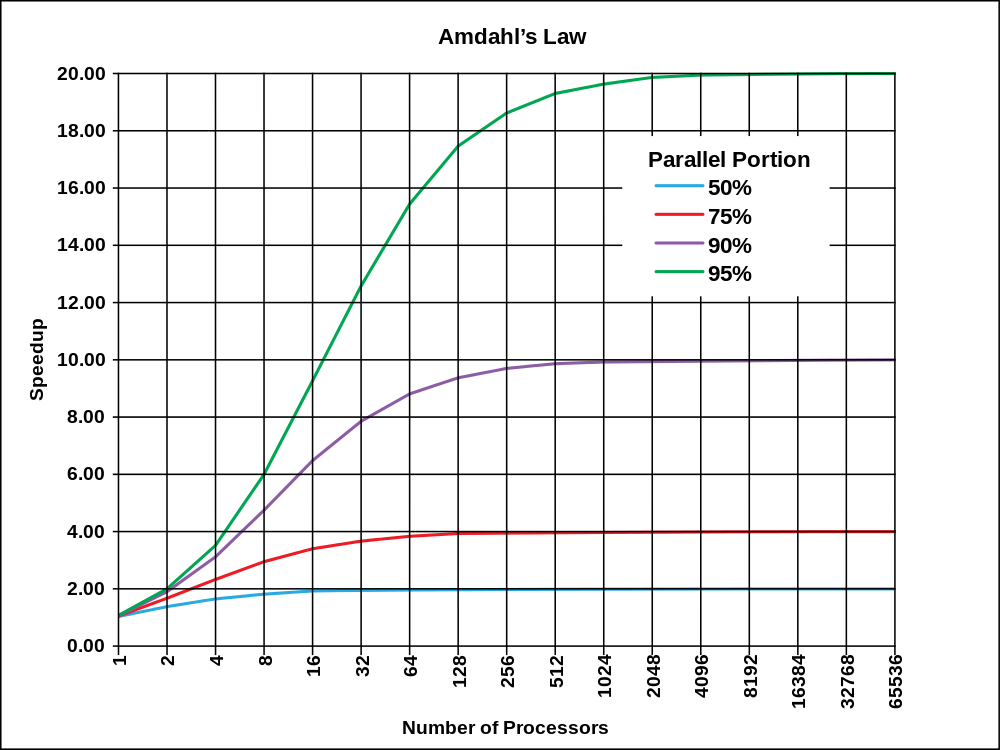
\includegraphics[width=11cm]{AmdahlsLaw.png}
    \caption{Illustration of Amdahls Law. Wikipedia Commons}
    \label{fig:AmdahlsLaw}
\end{figure}

There are limitation to Amdahls Law since it makes a couple of assumptions.

\begin{itemize}
  \item The number of executing threads remain constant over the course of the program.
  \item The parallel portion has perfect speedup. Often not true due to shared resources,eg caches, memor bandwidth, and shared data.
  \item The parallel portion has infinite scaling, not true due to similar limits as above. More threads will not increase performance after a while or might even decrease it.
  \item There is no overhead for creation and destruction of threads.
  \item The length of the serial portion is independent of the number of threads. Often the serial work is to divided the work to the threads, this work will obviously increase as the number of threads go up. More threads can also lead to more communcation overhead.
  \item The serial portion can't be overlapped by the parallel parts. For instance with producer consumer type pattern the consumer could be strictly serial but the time it takes could be overlapped by the parallel producers.
\end{itemize}

This means it's most accurate with programs that are of the fork-join type. Eg serial parts and then matrix operations.\\
\\
Gustafsons Law is closely related to Amdahls Law and can in some ways be more accurate than Amdahls Law. It makes similar assumptions as Amdahls Law however it also makes two additiona statments. It states that problems tends to expand when provided with more computational power, eg increased precision by reducing grid size, high frame rate for graphics. The second is that the parallel portion of the program tends to exapand faster than the serial part, eg for matrix multiplication the initialisation scales linearly with the matrix size while the multiplication itself scales as $O(n^3)$. The former means that it's closely realted to weak scaling. So in a way it says that the execution time remains constant rather than the ammount of data. More precise it says that the expected speedup with p threads and F fraction of the code that is parallel is\cite{gustafson1988reevaluating, cuda_best_practice}
$$S(p)=p+(1-F)(1-p)$$

\begin{figure}[h]
    \centering
    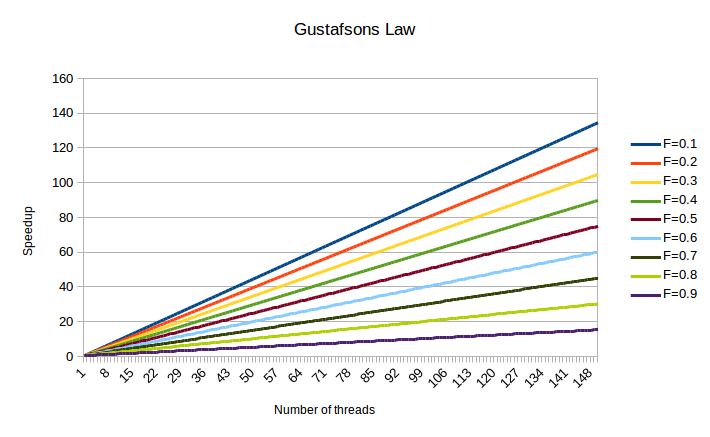
\includegraphics[width=13cm]{GustafsonsLaw.png}
    \caption{Illustration of Gustafsons Law}
    \label{fig:GustafsonsLaw}
\end{figure}

%\subsubsection{Profilers}
There are applications called profilers that are made to assses the programs performance and resource consumption. They calculate some of the measures mentioned above and they also check hardware usage and how much time the program spends at various parts of the program. This is very useful for finding bottlnecks and other problems in the program. It doesn't matter if the algorithm is super fast if all the data is stuck in network transfers. The profilers can be hardware dependent so the manufactures usually provided them for their products. For instance NVIDIA provides profilers for programs that use CUDA.\cite{introduction_hpc_hager, cuda_best_practice}

\clearpage
\subsection{Computer Architecture}
Most computers today have a multicore architecture
means several processors share the main memory and othe reaousrces. they can coperate on the same problem but it they are cordinated on a case by case basis since each algorithm requires different sharing.

Von Neuman architecture
It was first used in EDVAC which was one of the first stored program computers\cite{von1993first}. Stored programc computers uses electronic memory to store the program instructions\cite{computer_arch_2003}.

\begin{figure}[h]
    \centering
    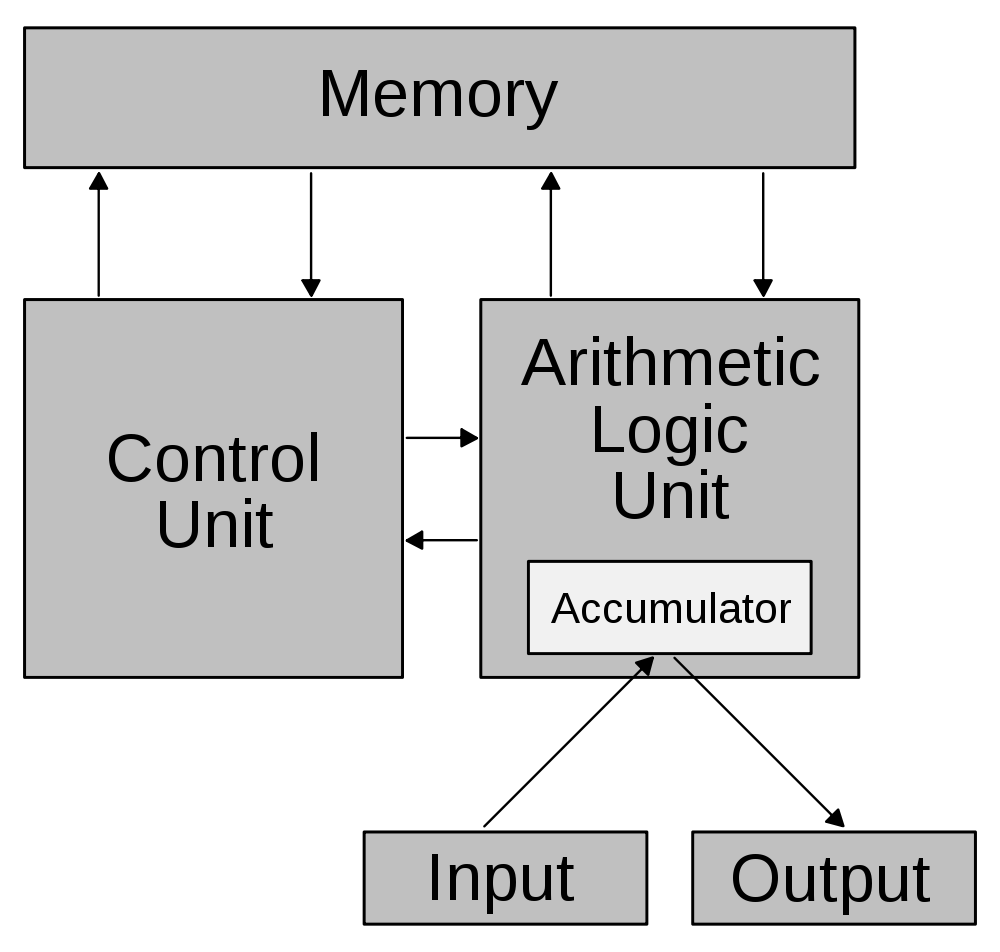
\includegraphics[width=7cm]{Von_Neumann_architecture.png}
    \caption{Schematic of the Von Neuman architecture. Wikipedia Commons}
    \label{fig:VonNeuman}
\end{figure}

blabla some text here about von neaum architecture

For HPC it's easiest to think about the architecture as three main parts, data storage, processor and the memory.\cite{intro_hpc}

\subsubsection{CPU}
Central processing unit(CPU) is \cite{introduction_hpc_hager}

Until 1996 there was computers with just a single core CPU on top 500\cite{TOP500}. Since about 2005 most desktop computers CPU has several cores which has increased the need for parallelization. The cores themselves aren't getting faster, the CPUs have more cores.

schematic here

branch prediction
prefetching

gpus might be hard but cpus aren't trivial either for HPC
parallelization isn't that easy either, depends on problem
correct use of caches is very important\cite{drepper2007cpumemory}

\subsubsection{Accelerators, GPU and Xeon Phi}
Graphics processing unit(GPU) have become more popular for general computing the last 10 years.

\begin{figure}[h]
    \centering
    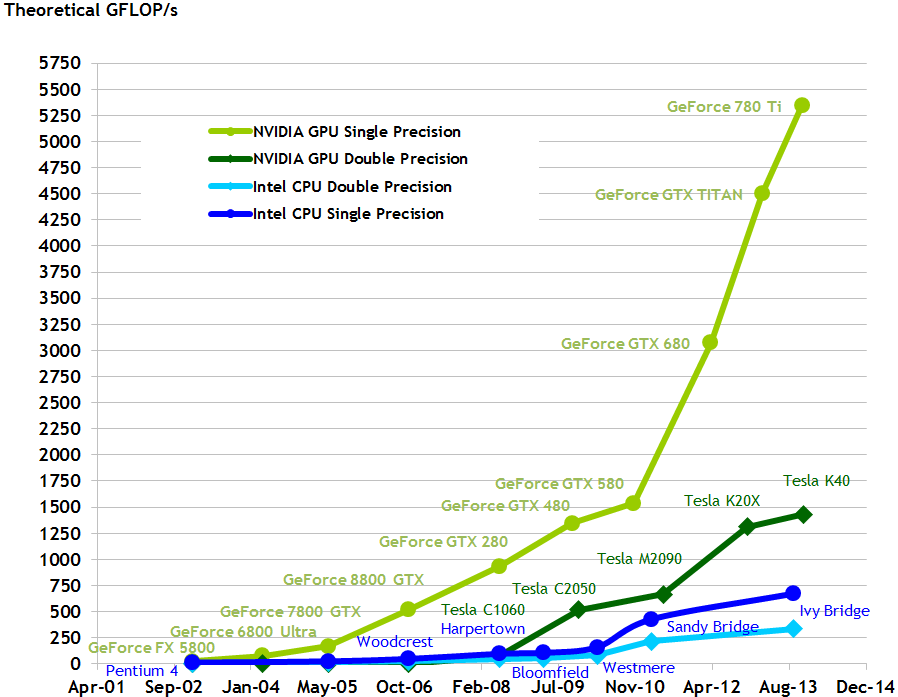
\includegraphics[width=11cm]{floating-point-operations-per-second.png}
    \caption{Bla bla \cite{cuda}}
    \label{fig:gpu_vs_cpu}
\end{figure}

something about single and double precision

structure of gpu

Xeon Phi, intel mic
mimd
knights landing, interesting new development from intel.
however usually but not always require mem copy
still need vectorisation and other stuff
you end up with similar problems
might be useful for old serial legacy code, but you still ned to parallelize it to get speed

structure of mic

\subsubsection{Which program for GPU and which for CPU?}
\label{gpu_gwas}
This a big question. As with a lot of things it depends on the algorithm to implement etc.

NVIDIA vs Intel performance claims, intel gets much lower than Nvidia. But who can you trust really?

If you have lots of legacy code then then you might need to rewrite a lot. However by using a profiler the parts that take up the most time can be found and moved to the GPU. However that migh be hard if the program isn't properly structured. No legacy code can also be a good thing. Old code might not be written with modern standards or use new nifty features and therefore lose speed.

Xeon Phi is an altnerative, simpler but can still be tricky and require mem copy.

GPUs loses more when going from single precision to double than CPUs. Peak performance on tesla-kepler cards for single precision is around 4 Tflops while double precision is around 1.4 Tflops. \cite{nvtesla}\\ ref the table thing how well does phi do?

In short GPUs excel at linear algebra but Intel MIC is probably a good alternative for it to.

GPUs are good for interaction algorithms since most approaches are embarasingly parallel since they consider each combination independtly from the others. They also often perform a lot of linear algebra. Several studies got high gains from implementing their programs on GPU, however their CPU versions weren't parallelized so it's likely that the gains would have been less compared to an optimized and parallelized CPU version.\cite{gwis,gboost,gmdr_gpu,cuda_lr,genie_2012,plink_gpu} However one study made a CPU cluster version and a GPU version of an algorithm that uses $chi^2$ tests, they found that 16 CPU nodes had the same performance as a single GTX 280 card\cite{jiang_accelerating}.%\\
%\\
%Possible exceptions could be algorithms that considers all combinations together since they would need more communcation.

\subsubsection{Clusters}
Clusters are collections of computers that can work together in several ways and are so tightly connected that they can usually be viewed as a single system. They communciate over a shared network but have seperate memory and procesors. Storage is usually shared. A computer in a cluster is called a \emph{node}. \cite{intro_hpc, kirk2012programming}

top 500\cite{TOP500}

Few clusters used GPUs before 2009 but now mix of GPUs and cpu are common among the top clusters. It was driven largely by demand for power saving while still giving high performance. The GPUs can do the heavy computation while other parts are used on CPU. Most of these clusters are hightly ranked in Green 500. \cite{kirk2012programming}

Flops is not everything, bad performace compare to theortical maximum
Stuck in network, harddrives, etc. Latency
Very few programs scale to the fastest clusters, peta scale.

Tianhe 2 is current top. Theoretical performance 54.9 PetaFlops.\cite{TOP500}
Max achived with LinPack 33 PetaFlops
60\% efficiency

Picture of Tianhe-2 here

mpi is commonly used for clusters\cite{kirk2012programming}

\subsection{CUDA programming model}
warps threads and stuff about CUDA\cite{cuda}

SIMT

blocks

\begin{figure}[h]
    \centering
    \includegraphics[width=10cm]{automatic-scalability.png}
    \caption{Blocks blocks blocks PlaceHolder picture. Need to make a black white verison}
    \label{fig:blocks_scaling}
\end{figure}

Hetrogenous programming model is used when seperate memory for CPU and GPU.

\subsubsection{Efficient CUDA}
One of the main critizm against GPUs for general computing purposes is that it's hard to get good performance because it requires good knowledge about details of the GPU architecture, especially the memory architecture. Here are somethings that needs to be considered when writing GPU programs.\cite{plink_gpu, cuda, cuda_best_practice}
\\
\begin{description}
  \item[Maximize parallelism] \hfill \\
  Structure the program and the algorithm in such a way that it's as parallel as possible and overlap the serial parts on CPU with calculations on the GPU.\cite{plink_gpu, cuda}
  \item[Minimize transfers between host and device] \hfill \\
  Moving data between host and device is expensive and should be avoided if possible. It can be better to run serial parts on the GPU rather than moving the data to the host to do the calculation on the CPU. The bandwidth between host and device is one of the large performance bottlnecks. This can be a problem when the data is to large to fit in the relativly small GPU dram.\cite{cuda, cuda_best_practice}
  \item[Find the optimal number of blocks and threads] \hfill \\
  There are a lot of things affected by the number of blocks and threads so they should be considered carefully. It's a good idea to parameterize them so that they can be changed for future hardware and varied for optimization. NVIDIA has an occupancy calculator which can be helpful in determining the optimal numbers, however high occupancy doesn't mean high performance.\cite{cuda, cuda_best_practice}\\
  \\
  The number of blocks should be larger than the number of multiprocessors so that all multiprocessors have atleast one block to execute. Having two blocks or more per multiprocessor can be good so that there are blocks that aren't waiting for a \_\_syncthreads() that can be executed. However this is not always possible due to shared memory usage and similar.\cite{cuda_best_practice}\\
  \\  
  The number of threads per block should be a multiplier of 32 but minimum 64. It's also important to rember that multiple concurrent blocks can reside on the same multiprocessor. To large number of threads in a block and parts of the multiprocessor might be idle since there aren't a block small enough to use those threads. Between 128 and 256 threads is a good place to start.\cite{cuda_best_practice}
  \item[Streams, concurrent kernels and asynchronous memory] \hfill \\
  By using streams it's possible to overlap memory transfers with calculations. This means that the data for the next batch can be transfered while the current batch is calculated and when it's done it can start calculating on the next batch directly after the current one is done. This can hide the time for transfers completly in some situations. However it requires the memory on the host to be pinned. Pinning to much memory can reduce performance of the host.\cite{cuda}\\
  \\
  Operations on a stream is guaranted to be done in the order they are made however calls on different streams can be executed in any order. Some GPUs allow kernels from different streams to be executed concurrently which can be a big boost if the kernels are to small to allocate most of the GPUs resources. Upto 16 or 32 kernels can be executed at the same time depending on GPU.\cite{cuda}
  \item[Use the correct memory on the GPU] \hfill \\
  Correct use of caches and memory is important for CPU\cite{drepper2007cpumemory}. It's also imporant on GPUs but it gets more complicated since the caches are smaller and there are several types of memory.
    \begin{itemize}
    \item Global memory is the main memory of the GPU and is accessible from all threads and blocks. However it's relativly slow to access.
    \item Shared memory is shared insided a block and is faster than global memory. However it's limited in size.
    \item Constant memory is small however its cached so it's fast to access. It's read only and best used for small amount of variables that all threads access.
    \item Local memory is tied to the threads scope, but it's still resides off-chip so it has the same access time as global memory.
    \item Texture memory is read only and can be faster to access than global memory in some situations. This was more important in older GPUs when global memory wasn't cached.\cite{plink_gpu, cuda}
  \end{itemize}
  \item[Avoid divergence] \hfill \\
  Each thread in a warp executes the same instruction at the same time so if some of threads diverge the rest will be ideal until they are at the same instruction again. This means it's important to use control strucutres such as if statments carefully to prevent threads from idiling.\cite{cuda, cuda_best_practice}
  \item[Avoid memory bank conflicts when using shared memory] \hfill \\
  Shared memory is divided into equally-sized memory modules called banks that can be accessed at the same time for higher bandwidth. Bank conflicts occur when seperate threads access the same bank. Bank conflicts are split into as many conflict-free requests as needed.\cite{cuda, cuda_best_practice}
  \item[Use existing libraries] \hfill \\
  Instead of writing everything from scratch it's usually a good idea to use already existing libraries. Espeically when performance is important and most task are non trivial on GPUs so using an already optimized library is a good idea. Some of the most popular libraries for CUDA are:
  \begin{itemize}
    \item CUBLAS: BLAS implementation for CUDA\cite{cublas}
    \item CULAtools: BLAS and LAPACK implementation for CUDA for both dense and sparse matrices\cite{culatools}
    \item MAGMA: BLAS and LAPACK implementation among other things that can distribute the work on both CPU and GPU\cite{magma_2010}
    \item Thrust: Template based library that tries to emulate C++ standard library\cite{thrust_gpu}
  \end{itemize}
  \item[Avoid slow instructions] \hfill \\
  There are some instructions that can be slow and should be avoided if possible, for instance type conversion, integer division and modulo. If a function is called with a floating point number that might be used as a double and require a conversion. By putting an f at the end of the number it's told to be single precision float, for instance 0.5f. In some cases it's possible to use bitwise operations instead which is faster.\cite{cuda, cuda_best_practice}
  \item[Restricted pointers can give increased performance] \hfill \\
  Aliasing is a problem in some languages, it occures when two pointers point to the same place in memory and the code does operations on them at the same place. This means that operations that look like they can be done in any order actually can't and thus prevents the compiler to make optimizations. The problem is that the compiler has to take this in to account for all pointers even if no aliasing occurs because it might happen. By using the \_\_restrict\_\_ keyword on pointers the compiler can be told that no aliasing will occur, however it's up to the programmer to make sure that is the case or there might be strange results. Not using aliasing reduces the number of memory accesses the CPU needs to make. However it increases register pressure so it can have an negative effect on performance.\cite{cuda} Aliasing can be important to keep in mind for CPU code as well\cite{drepper2007cpumemory}.
  \item[Use fast math functions if precision isn't needed] \hfill \\
  There are two versions of runtime math functions. The ones of the type funcf() is slower but more accurate than \_funcf(). The option -use\_fast\_math makes the compiler change all the funcf() to \_funcf().\cite{cuda_best_practice}
\end{description}

TODO
Some stuff for multi gpu
They dont share memory.

unrolling is really good, see volkovs stuff

\clearpage
\section{Algorithm}
%Algorithm (up till 20 pages)
%  - Current state - Basic algorithm, Data structure, memory consumption, parallelization, load balancing and scalability
%  - And the same for own your implementation

%TODO nån typ av intro här

%OTHERS
%problem with exathsutive

%memory problems(GENIE, CUDALR and so on)

%2 bit 3 bit data storage

%two stage analysis


\subsection{Current algorithm}
JEIRA uses Java and it's built-in functions for concurrency.

Producer consumer pattern

Strucuture picture here.

Symmetric condfidence interval of additive effects.

%\subsection{Mine}
%exhaustive and second stage.

\section{Results}
%Results (up till 15 pages including plots)
%  - Performance measurements (scalability, speedup and efficiency as well as load balancing)
%  - Setup(simulation setup, compilers and hardware setup)
%  - Single node performance
%  - multy-node performance


\section{Discussion and Conclusions}
%Discussion and Conclusions (up to 3 pages)
Need for novel methods for gene-enviroment interaction
Need for methods for third order interaction or higher, for both gene-gene and gene-enviroment

\section{Outlook}
%Outlook (up to one page)

\section{Appendix}
%List of figs
%List of tables


\newpage
\bibliographystyle{ieeetr}
\bibliography{hpc.bib,statistics.bib,misc.bib}
\end{document}